% !TEX root = ../SinkhornDivergenceUnbalanced.tex


\section{The Sinkhorn algorithm and its convergence}
\label{sec-sinkhorn}

We now present a reformulation of the Sinkhorn algorithm to the unbalanced setting, first introduced in~\cite{chizat2016scaling}.
Crucially, the novelty is the introduction of $\aprox{\phi^*}$, which allows to prove convergence for a variety of settings.
Our general formalism allows to consider positive Radon measures.
So far convergence was only proved for discrete measures when $\D_\phi=\iota_{(=)}$ or $\rho\KL$~\cite{chizat2016scaling} via the non-linear Perron Frobenius theory~\cite{lemmens2012nonlinear}.
We emphasize that our reformulation also leads to a numerically stable algorithm, see Section~\ref{sec-implementation}.
%
%This original formulation allows us to overcome the limitations of earlier proofs of convergence for the Sinkhorn algorithm, that were based on the theory of non-linear Perron Frobenius operators~\cite{lemmens2012nonlinear} and only hold for balanced OT and unbalanced OT with a KL divergence.
%%
%Our results hold in much larger generality and allow us to study a collection
%of popular models for unbalanced OT within a common theoretical and algorithmic framework.



\subsection{Sinkhorn iterations}

The Sinkhorn algorithm aims at solving the dual problem of $\OTb(\al,\be)$, which reads $\OTb(\al,\be)
=\sup_{(\f, \g)\in \Cc(\Xx)^2}\Ff(\f,\g)$, where
\begin{equation} \label{eq-dual-unb}
\Ff(\f,\g) \eqdef
- \dotp{\al}{\phi^*(-\f)}
- \dotp{\be}{\phi^*(-\g)}
-\epsilon \dotp{\al\otimes\be}{\fefgc - 1},
\end{equation}
and $\phi^*$ is the Legendre transform of $\phi$.
%
This problem is equivalent to Problem~\eqref{eq-primal-unb} thanks to Fenchel-Rockafellar theorem.
%
The variables $(\f,\g)$ are called \emph{dual potentials}.
%
The optimal plan $\pi$ and optimal $(\f,\g)$ are connected via the primal-dual optimality relation
%
\begin{align} \label{eq-implicit-plan}
\pi(x,y) ~&=~ \exp\big[\tfrac{1}{\epsilon}(\f(x)+ \g(y) - \C(x,y))\big]\al(x)\be(y) ~\in~ \Mmp(\Xx\times\Xx).
\end{align}

%\end{align}

%As detailed for instance in \cite[Section 3.3.1]{feydy2020thesis}, the Sinkhorn algorithm is derived as a block-coordinate ascent method on this dual problem.
%%
%Crucially, we split its iterations in two steps using the Softmin and anisotropic prox operators:

We present the dual optimality conditions. They involve the operators presented Section~\ref{sec-operators}.

\begin{proposition}[Optimality conditions for the dual problem]\label{prop-optimality-prox}
The first order optimality condition of Formulation~\eqref{eq-dual-unb} reads
\begin{gather}\label{eq-optim-cond}
	\begin{aligned}
	\f(x) &= -\aprox{\phi^*}\big(-\Ss_\be(\g)(x)\big),\quad \al-\text{a.e.} \\
	\g(y) &= -\aprox{\phi^*}\big(-\Ss_\al(\f)(y)\big), \quad \be-\text{a.e.},
	\end{aligned}
\end{gather}
where $\aprox{\phi^*}$ is applied pointwise, and $(\Ss_\al,\Ss_\be)$ are defined Equation~\eqref{eq-defn-softmin-func}.
For the sake of brevity, we define operators $(\Aa\Ss_\al,\Aa\Ss_\be)$ outputing functions in $\Cc(\Xx)$ to write Equations~\eqref{eq-optim-cond} as $\f =  \Aa\Ss_\be(\g)$ and $\g=\Aa\Ss_\al(\f)$.
\end{proposition}
%
\begin{proof}
The first order conditions on $\partial_\f\Ff(\f,\g)$ and $\partial_\g\Ff(\f,\g)$ read
\begin{align} \label{eq-dual-optimality}
e^{\frac{\f}{\epsilon}}\dotp{\be}{e^{\frac{( \g - \C )}{\epsilon}}} \in \partial\phi^*(-\f),\, \al\text{-a.e.}
\;\;\;\; \text{and} \;\;\;\;
e^{\frac{\g}{\epsilon}}\dotp{\al}{e^{\frac{( \f - \C )}{\epsilon}}} \in \partial\phi^*(-\g), \, \be\text{-a.e.}
\end{align}
One has $e^{-\Smin{\be}(\C(y,.)-\g) / \epsilon} = \dotp{\be}{e^{\frac{( \g - \C )}{\epsilon}}}$. 
The optimality condition of $\aprox{\phi^*}$ (Equation~\eqref{eq-def-aprox}) is $e^{\frac{p - q}{\epsilon}} \in \partial\phi^*(q)$.
For any $y\in\Xx$, when $p=-\Smin{\be}(\C(y,.)-\g)$ or $p=-\Smin{\al}(\C(.,y)-\g)$ we retrieve Equation~\eqref{eq-dual-optimality} for $q = -\f$ or $q=-\g$. 
Hence the reformulation of Equation~\eqref{eq-dual-optimality} into Equation~\eqref{eq-optim-cond}.
\end{proof}

%A similar factorization was written in exponential form in~\cite{chizat2016scaling}, where the exponential analog of $\aprox{\phi^*}$ is called ``proxdiv" and reads
%\begin{align*}
%  e^{\frac{\f}{\epsilon}} = \text{proxdiv}^\epsilon_{\phi^*}(
%    k_\epsilon \star ( e^{\frac{\g}{\epsilon}} \be )
%  ),
%\end{align*}
%where $k_\epsilon = e^{-\C/\epsilon}$.
%
%The new factorization~\eqref{eq-optim-cond-1} is more appealing: it allows us to show in Section~\ref{sec-convergence} the contractance and regularity results that are at the heart of our convergence analysis for the algorithm.
%%
%As detailed in Section~\ref{sec-implementation}, it also lends itself better to numerically stable implementations on modern hardware.
%
\begin{remark}\label{rem-extrapolate-pot}
	Note that while Equations~\eqref{eq-optim-cond} only need to hold $(\al,\be)$-a.e. for optimality, they are well-defined for any $(x,y)\in\Xx^2$. It allows to extrapolate and define $(\f,\g)$ on the full space $\Xx$.
\end{remark}
%
One deduces Sinkhorn iterations from Proposition~\ref{prop-optimality-prox}, which perform an alternate dual maximization on $\Ff(\f,\g)$ by fixing one variable and optimizing the other.

\begin{definition}[Sinkhorn algorithm]
\label{def-sinkhorn}
Starting from some $\g_0 \in \Cc(\Xx)$, the iterations of Sinkhorn read
\begin{gather}
\begin{aligned}\label{eq-sinkhorn-iter-1}
\f_{t+1} &\eqdef \arg\max_{\f}\Ff(\f,\g_t)=\Aa\Ss_\be(\g_t),\\
\g_{t+1} &\eqdef  \arg\max_{\g}\Ff(\f_{t+1},\g)=\Aa\Ss_\al(\f_{t+1}).
\end{aligned}
\end{gather}
\end{definition}

%\begin{remark}\label{rem-pot-extrapolate}
%Note again that while the optimality conditions~\eqref{eq-dual-optimality} are only required to hold $(\al,\be)$ almost everywhere, the iterations define continuous functions on the whole space $\Xx$.
%\end{remark}

%
The $\aprox{\phi^*}$ is frequently known in closed form, has a small computational cost (see Section~\ref{sec-exmp-f-div}), and acts pointwise on e.g. $\Ss_\al(\f)$.
Thus the time and space complexity of iterations~\eqref{eq-sinkhorn-iter-1} is the same as balanced Sinkhorn, i.e. computing $(\Ss_\al,\Ss_\be)$ is the bottleneck scaling as $O(N^2)$. 
%The only modification needed to account for destruction and creation of mass is the \emph{pointwise} application of the aprox operator,
%at a negigible computational cost. We stress that in most useful settings, $\aprox{\phi^*}$ has a closed form expression that is presented in Section~\ref{sec-exmp-f-div}.

%In practice, $f\mapsto -\aprox{\phi^*}(-f)$ acts as a \emph{dampening} of the dual potentials that prevents the implicit transport plan
%$\pi = \exp[ (\f\oplus \g - \C) / \epsilon ] \cdot \al \otimes \be$
%encoded by the dual pair $(\f,\g)$ from saturating the mass transportation constraints.
%Section~\ref{sec-implementation} details an implementation of the algorithm for discrete measures, where the potentials $(\f,\g)$ are only computed $(\al,\be)$-a.e. and can thus be encoded as finite dimensional vectors.
%
%After convergence of this discrete algorithm, we can then use \eqref{eq-optim-cond-1} and~\eqref{eq-optim-cond-2} to extrapolate these dual vectors from the measures' supports to any point of the ambient space $\Xx$.


We end this section with a proof that a pair of potentials is optimal if and only if it is a fixed point of the Sinkhorn algorithm.

\begin{proposition}[Link between the Sinkhorn algorithm and the unbalanced $\OTb$ problem]\label{prop-cns-optimality}
A pair of dual potentials $(\f,\g)$ is optimal if and only if it is a fixed point of the Sinkhorn mapping.
\end{proposition}
\begin{proof}
Decompose the dual functional~\eqref{eq-dual-unb} as $\Ff(\f,\g) = \Ff_1(\f) + \Ff_2(\g) + \Ff_3(\f,\g)$ where $\Ff_1(\f)=\dotp{\al}{-\phi^*(-\f)}$, $\Ff_2(\f)=\dotp{\be}{-\phi^*(-\g)}$ and $\Ff_3(\f,\g)=-\epsilon \dotp{\al\otimes\be}{\fefgc - 1}$. For any function $\Gg$ one has $\partial\Gg(\f,\g) \subseteq \partial_1\Gg(\f,\g)\times\partial_2\Gg(\f,\g)$. Nevertheless for $\Gg(\f,\g)=\Ff_1(\f)+\Ff_2(\g)$ the inclusion of subgradients becomes an equality since it is a separable function in $(\f,\g)$. Furthermore, $\Ff_3$ is a differentiable function, thus the same equality between subgradients holds. Eventually, the subgradients can be summed because $\Ff_3$ is differentiable on $\R$, thus the intersection of subgradients is non-empty, and $\partial\Ff=\partial((\Ff_1 + \Ff_2) + \Ff_3) = \partial(\Ff_1 + \Ff_2) +   \partial\Ff_3 = \partial_1\Ff\times\partial_2\Ff$.

The condition $0\in\partial\Ff$ means that the dual variable are optimal, and $0\in\partial_1\Ff\times\partial_2\Ff$ that the potentials are fixed points of the Sinkhorn mapping. The equality between those two sets means that being optimal and being fixed points is equivalent.
\end{proof}



%\subsection{Summary of the method}
%\todo{Compress this section/remove}
%
%Before providing a theoretical analysis of the algorithm, let us recapitulate the main ingredients of the method. Table~\ref{tab-entropies-aprox} summarize the most important information.
%
%
%
%
%As detailed in~\eqref{eq-primal-unb}, unbalanced transport models are parameterized by a Csisz\'{a}r divergence $\D_\phi(\cdot|\cdot)$:
%  this penalty ensures that the marginals
%  $\pi_1 = \pi \mathbf{1}$ and $\pi_2 = \t{\pi} \mathbf{1}$
%  of the transport plan $\pi$
%  remain close to the input measures $\al$ and $\be$.
%  The (soft) mass transportation constraints in the transport problem
%  are encoded by an entropy function $\phi$ which is
%  applied to the relative densities $\tfrac{\d \pi_1}{\d \al}$
%  and $\tfrac{\d \pi_2}{\d \be} \geq 0$ and penalizes deviations
%  to the desired value of $1$. \protect
%
%With Definition~\ref{def-sinkhorn} and Theorem~\ref{thm-cv-sink-compact},
%  we show that unbalanced OT problems can be solved
%  using successive applications of a Softmin operator
%  and a function $p\mapsto -\aprox{\phi^*}(-p)$
%  on the dual potentials $\f$ and $\g$.
%  In the standard \emph{balanced}
%  setting, which corresponds to a strong equality constraint on the marginals,
%  this second operation is the identity operator $p\mapsto p$
%  and we retrieve the standard \textbf{Sinkhorn iterations}.
%  In other settings, illustrated in Figure~\ref{fig-aprox}, we retrieve 1-Lipschitz functions
%  such as a Soft Thresholding (Range setting),
%  a Clamp operation (TV setting)
%  or a multiplication by a scalar $\tfrac{\rho}{\rho + \epsilon} < 1$ (KL setting).
%
%  We understand the pointwise application
%  of this operator as a \textbf{dampening} of
%  the dual potentials $\f$ and $\g$ that allows the implicit transport plan
%  $\pi = \exp\tfrac{1}{\epsilon}[\f\oplus \g - \C]\cdot (\al\otimes \be)$
%  to ignore pairs of points $x$, $y$ in the supports of $\al$ and $\be$
%  for which $\C(x,y)$ is too large to warrant transport over mass creation and destruction.
%  In an algorithmic sense,
%  \textbf{unbalanced OT can thus be understood as the theory
%  that justifies the application of pointwise ``non-linearities''
%  between the iterations of the Sinkhorn algorithm}.
%  This ``trick'' is in line with many
%  similar methods in the deep learning literature \cite{WassersteinGAN}
%  and allows practitioners to make their transport plans robust to outlier samples
%  at a negligible computational cost.




\subsection{Examples of Csiszár divergences}
\label{sec-exmp-f-div}

We present now explicit settings, and provide in each case $(\phi,\phi^*,\aprox{\phi^*})$. 
Those settings correspond to different priors on mass variation dynamics. 
We provide below illustrations of $\aprox{\phi^*}$ and the influence of $\phi$ on $\OTb$.


\paragraph{Balanced OT} ($\D_\phi=\iota_{(=)}$) corresponds to using $\phi = \iota_{\{1\}}$, the convex indicator function which encodes the marginal constraints, i.e. $\frac{\d\pi_1}{\d\al} = 1$ and $\frac{\d\pi_2}{\d\be} = 1$. In this case we get $\phi^*(q) = q$ and $\aprox{\phi^*}(p) = p$.


\paragraph{Kullback-Leibler} ($\D_\phi=\rho\KL$) corresponds to $\phi(p) = \rho ( p \log p -p +1)$, to $\phi^*(q) = \rho(e^{q / \rho} -1)$ and $\aprox{\phi^*}(p) = (1+\tfrac{\epsilon}{\rho})^{-1} p$.
%
As discussed in \cite{liero2015optimal}, when $\epsilon=0$ and $d_\Xx$ a distance, unbalanced OT defines the Gaussian-Hellinger and the Kantorovitch-Hellinger distances on $\Mmp(\Xx)$ (respectively for $\C(x,y)=d_\Xx(x,y)^2$ and $\C(x,y)=-2\log\cos(d_\Xx(x,y)\wedge\pi))$).


\paragraph{Range} ($\D_\phi=RG_{[a,b]}$) is defined for $0\leq a \leq 1 \leq b$ with $\phi = \iota_{[a,b]}$ and $\phi^*(q) = \max(a q, b q)$. The proximal operator is
\begin{align*}
\aprox{\phi^*}(p) =
\text{Soft-Thresh}_{\epsilon \log a}^{\epsilon \log b}(p)=
\begin{cases}
p - \epsilon\log a & \quad\text{if } p - \epsilon\log a < 0,\\
p - \epsilon\log b & \quad\text{if } p - \epsilon\log b > 0,\\
0 & \quad\text{otherwise.}
\end{cases}
\end{align*}
Note that in this setting the problem can be infeasible, i.e. $\OTb(\al,\be)=+\infty$. We have $\OTb(\al,\be)<\infty$ if and only if $[m(\al)a,m(\al)b]\cap[m(\be)a,m(\be)b]\neq\emptyset$.
\begin{proof}
	Take $(\al,\be)$ such that $m(\al)b < m(\be)a$. The range penalty imposes on the primal $m(\al)a \leq m(\pi) \leq m(\al)b$ and $m(\be)b \leq m(\pi) \leq m(\be)b$, which is infeasible. A similar proof holds if $m(\be)b < m(\al)a$.
	%
	Conversely, take $k\in[m(\al)a,m(\al)b]\cap[m(\be)a,m(\be)b]\neq\emptyset$. Then one can verify that $\pi=(k / m(\al)m(\be))\al\otimes\be$ is a feasible plan, which guarantees that both the primal and the dual are finite.
\end{proof}

\paragraph{Total Variation} ($\D_\phi=\rho TV$) corresponds to $\phi(p) = \rho|p-1|$ and for $q\leq \rho$, $\phi^*(q) = \max(-\rho, q)$ with $\text{dom}(\phi^*) = (-\infty, \rho]$. The anisotropic operator reads
\begin{align*}
\aprox{\phi^*}(p) =
\text{Clamp}_{[-\rho, +\rho]}(p)=
\begin{cases}
-\rho & \quad\text{if } p < -\rho \\
p & \quad\text{if } p \in [-\rho, \rho]\\
\rho & \quad\text{if } p > \rho.
\end{cases}
\end{align*}
In this case, unbalanced OT (i.e. when $\epsilon=0$) is a Lagrangian version of partial optimal transport~\cite{figalli2010optimal}, where only some fraction of the total mass is transported. 
When $\C$ is a distance, it is also equivalent to the flat norm (the dual norm of bounded Lipschitz functions)~\cite{hanin1999extension,hanin1992kantorovich,schmitzer2019framework}.

\paragraph{Power entropies} divergences are parametrized by $s\in\R\setminus\{0,1\}$ and $r \eqdef s / (s-1)$. When $s<1$ it correspond to
\begin{align*}
\phi(p) = \frac{\rho}{s(s-1)}\big(p^s -s(p-1) -1 \big) \qandq 
\phi^*(q) = \rho\frac{r-1}{r}\left[\big(1 + \frac{q}{\rho(r-1)}\big)^r -1\right].
\end{align*}
Special cases include \emph{Hellinger} with $s=1/2$, and \emph{Berg entropy} as the limit case $s=0$, defined by $\phi(p) = \rho(p - 1 - \log p)$ and $\phi^*(q) = - \rho\log( 1 - q / \rho)$ with $\text{dom}(\phi^*) = (-\infty, \rho)$. 
Kullback-Leibler is the limit $s=1$. 
We refer to~\cite{liero2015optimal} for more details.
%When $s<1$ and $s\neq 0$, the conjugate exponent is $r \eqdef s / (s-1)$ and the Legendre transform reads
The following proposition summarizes important properties of this divergence needed for the analysis of Sinkhorn interates.


\begin{proposition}[Properties of the power entropy]\label{prop-aprox-power-ent}
	For any dual exponent $r<1$, $\phi^*$ is strictly convex and $\partial\phi^*(x)\rightarrow 0$ when $x\rightarrow -\infty$. The proximal operator satisfies
	\begin{align}\label{eq-lambert}
	\aprox{\phi^*}(p) = \rho(1-r) - \epsilon (1-r) W\left(\frac{\rho}{\epsilon} \exp\big(\frac{-p + \rho(1-r)}{\epsilon(1-r)}\big)\right),
	\end{align}
	where $W$ is the Lambert function, which satisfies for any $p\in\R_+$ $W(p)e^{W(p)} = p$, see~\cite{corless1996lambertw}.
	%
	It is a non-expansive operator, and it is a contraction on compact sets.
\end{proposition}

\begin{proof}
	The strict convexity and the limit of the gradient is immediate.
	For any input $p$, $q = \aprox{\phi^*}(p)$ satisfies
	\begin{align*}
	& e^{\tfrac{p-q}{\epsilon}} = (1 - \tfrac{q}{\rho(1-r)})^{r-1}\\
	&\Leftrightarrow \quad  \epsilon(1-r) \log(1 - \tfrac{q}{\rho(1-r)}) + p - q = 0 \\
	&\Leftrightarrow \quad \epsilon(1-r)\log(Q) + \rho(1-r) Q + (p -\rho(1-r)) = 0 \text{  with  } Q = 1 - \tfrac{q}{\rho(1-r)}\\
	&\Leftrightarrow \quad q(p) = \rho(1-r) - \epsilon (1-r) W(\Delta(p))
	\text{  with  } \Delta(p) = \tfrac{\rho}{\epsilon}e^{\frac{-p + \rho(1-r)}{\epsilon(1-r)}}.
	\end{align*}
	We now show that the above mapping is indeed 1-Lipschitz. We first note that $\frac{\d\Delta}{\d p} = -\frac{\Delta(p)}{(1-r)\epsilon}$. The derivative of the Lambert function gives
	\begin{align*}
	\frac{\d q(p)}{\d p} = -\epsilon(1-r) \frac{\d\Delta}{\d p}\frac{\d W}{\d \Delta} = \epsilon(1-r) \frac{\Delta}{\epsilon(1-r)} \frac{W(\Delta)}{\Delta(1 + W(\Delta))}= \frac{W(\Delta)}{(1 + W(\Delta))} <1.
	\end{align*}
	Because $\Delta(p) >0$ we have $W(\Delta)\geq 0$, and $W(\Delta)\rightarrow +\infty$ when $p\rightarrow -\infty$. 
	Thus $\aprox{\phi^*}$ is 1-lipschitz and contractive when iterations are restricted to a compact set.
\end{proof}

Note that Formula~\eqref{eq-lambert} enables a fast evaluation of $\aprox{\phi^*}$. 
The Lambert function is computable via the cubically converging Halley's algorithm~\cite{alefeld1981convergence}. 
It is also computable on GPU devices.



\begin{figure}[p]
	\begin{minipage}{\textwidth}
	\centering
	%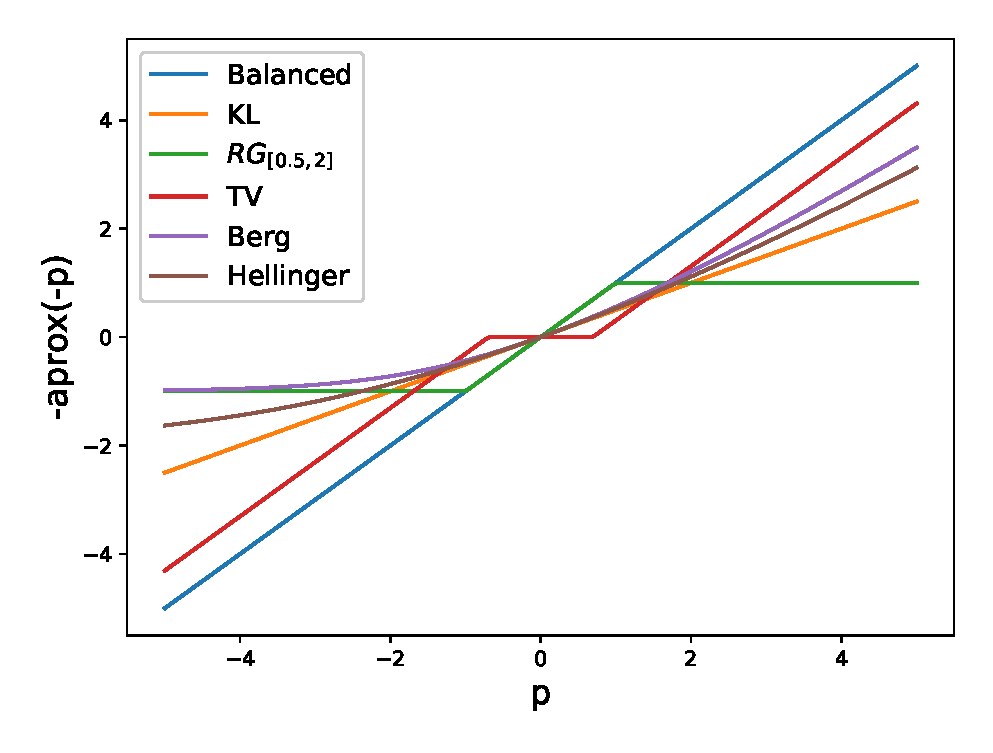
\includegraphics[width=.5\linewidth]{images/fig_aprox_5}
	\resizebox{!}{5cm}{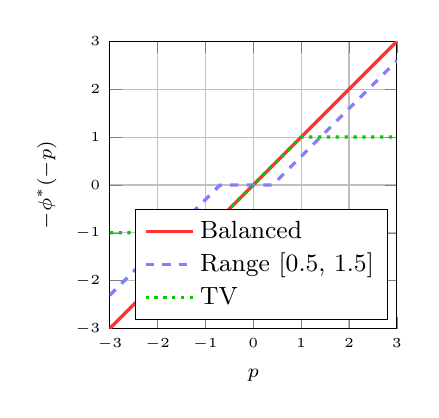
\begin{tikzpicture}
\iffalse
import sys
import numpy as np
p = np.linspace(-3, 3, 121)
a, b = 0.5, 1.5
eps, rho = 1, 1

# Range
range = p.copy()
range[p < eps * np.log(a)] -= eps * np.log(a)
range[(p >= eps * np.log(a)) * (p <= eps * np.log(b))] = 0
range[p > eps * np.log(b)] -= eps * np.log(b)

# TV
tv = p.copy()
tv[p < -rho] = -rho
tv[p > rho] = rho

values = np.stack((p, p, range, tv)).T
np.savetxt(sys.stdout, values, fmt="%.3f")
\fi

    \pgfplotstableread{
    p balanced range tv
    -3.000 -3.000 -2.307 -1.000
    -2.950 -2.950 -2.257 -1.000
    -2.900 -2.900 -2.207 -1.000
    -2.850 -2.850 -2.157 -1.000
    -2.800 -2.800 -2.107 -1.000
    -2.750 -2.750 -2.057 -1.000
    -2.700 -2.700 -2.007 -1.000
    -2.650 -2.650 -1.957 -1.000
    -2.600 -2.600 -1.907 -1.000
    -2.550 -2.550 -1.857 -1.000
    -2.500 -2.500 -1.807 -1.000
    -2.450 -2.450 -1.757 -1.000
    -2.400 -2.400 -1.707 -1.000
    -2.350 -2.350 -1.657 -1.000
    -2.300 -2.300 -1.607 -1.000
    -2.250 -2.250 -1.557 -1.000
    -2.200 -2.200 -1.507 -1.000
    -2.150 -2.150 -1.457 -1.000
    -2.100 -2.100 -1.407 -1.000
    -2.050 -2.050 -1.357 -1.000
    -2.000 -2.000 -1.307 -1.000
    -1.950 -1.950 -1.257 -1.000
    -1.900 -1.900 -1.207 -1.000
    -1.850 -1.850 -1.157 -1.000
    -1.800 -1.800 -1.107 -1.000
    -1.750 -1.750 -1.057 -1.000
    -1.700 -1.700 -1.007 -1.000
    -1.650 -1.650 -0.957 -1.000
    -1.600 -1.600 -0.907 -1.000
    -1.550 -1.550 -0.857 -1.000
    -1.500 -1.500 -0.807 -1.000
    -1.450 -1.450 -0.757 -1.000
    -1.400 -1.400 -0.707 -1.000
    -1.350 -1.350 -0.657 -1.000
    -1.300 -1.300 -0.607 -1.000
    -1.250 -1.250 -0.557 -1.000
    -1.200 -1.200 -0.507 -1.000
    -1.150 -1.150 -0.457 -1.000
    -1.100 -1.100 -0.407 -1.000
    -1.050 -1.050 -0.357 -1.000
    -1.000 -1.000 -0.307 -1.000
    -0.950 -0.950 -0.257 -0.950
    -0.900 -0.900 -0.207 -0.900
    -0.850 -0.850 -0.157 -0.850
    -0.800 -0.800 -0.107 -0.800
    -0.750 -0.750 -0.057 -0.750
    -0.700 -0.700 -0.007 -0.700
    -0.650 -0.650 0.000 -0.650
    -0.600 -0.600 0.000 -0.600
    -0.550 -0.550 0.000 -0.550
    -0.500 -0.500 0.000 -0.500
    -0.450 -0.450 0.000 -0.450
    -0.400 -0.400 0.000 -0.400
    -0.350 -0.350 0.000 -0.350
    -0.300 -0.300 0.000 -0.300
    -0.250 -0.250 0.000 -0.250
    -0.200 -0.200 0.000 -0.200
    -0.150 -0.150 0.000 -0.150
    -0.100 -0.100 0.000 -0.100
    -0.050 -0.050 0.000 -0.050
    0.000 0.000 0.000 0.000
    0.050 0.050 0.000 0.050
    0.100 0.100 0.000 0.100
    0.150 0.150 0.000 0.150
    0.200 0.200 0.000 0.200
    0.250 0.250 0.000 0.250
    0.300 0.300 0.000 0.300
    0.350 0.350 0.000 0.350
    0.400 0.400 0.000 0.400
    0.450 0.450 0.045 0.450
    0.500 0.500 0.095 0.500
    0.550 0.550 0.145 0.550
    0.600 0.600 0.195 0.600
    0.650 0.650 0.245 0.650
    0.700 0.700 0.295 0.700
    0.750 0.750 0.345 0.750
    0.800 0.800 0.395 0.800
    0.850 0.850 0.445 0.850
    0.900 0.900 0.495 0.900
    0.950 0.950 0.545 0.950
    1.000 1.000 0.595 1.000
    1.050 1.050 0.645 1.000
    1.100 1.100 0.695 1.000
    1.150 1.150 0.745 1.000
    1.200 1.200 0.795 1.000
    1.250 1.250 0.845 1.000
    1.300 1.300 0.895 1.000
    1.350 1.350 0.945 1.000
    1.400 1.400 0.995 1.000
    1.450 1.450 1.045 1.000
    1.500 1.500 1.095 1.000
    1.550 1.550 1.145 1.000
    1.600 1.600 1.195 1.000
    1.650 1.650 1.245 1.000
    1.700 1.700 1.295 1.000
    1.750 1.750 1.345 1.000
    1.800 1.800 1.395 1.000
    1.850 1.850 1.445 1.000
    1.900 1.900 1.495 1.000
    1.950 1.950 1.545 1.000
    2.000 2.000 1.595 1.000
    2.050 2.050 1.645 1.000
    2.100 2.100 1.695 1.000
    2.150 2.150 1.745 1.000
    2.200 2.200 1.795 1.000
    2.250 2.250 1.845 1.000
    2.300 2.300 1.895 1.000
    2.350 2.350 1.945 1.000
    2.400 2.400 1.995 1.000
    2.450 2.450 2.045 1.000
    2.500 2.500 2.095 1.000
    2.550 2.550 2.145 1.000
    2.600 2.600 2.195 1.000
    2.650 2.650 2.245 1.000
    2.700 2.700 2.295 1.000
    2.750 2.750 2.345 1.000
    2.800 2.800 2.395 1.000
    2.850 2.850 2.445 1.000
    2.900 2.900 2.495 1.000
    2.950 2.950 2.545 1.000
    3.000 3.000 2.595 1.000
    }\datatable
          
  
  \begin{axis}[width=.5\textwidth,
              grid=both,ymin=-3, ymax=3, xmin=-3, xmax=3,
      %title={\scriptsize We run NumPy, PyTorch and KeOps on a RTX 2080 Ti GPU.},
              xlabel={\scriptsize $p$}, 
              ylabel={\scriptsize $-\aprox{\phi^*}(-p)$}, 
              xtick={-3,-2,-1,0,1,2,3},
              %xticklabels={100,1k,10k,100k,1M},
              ytick={-3,-2,-1,0,1,2,3},
              %yticklabels={1\,ms,10\,ms,100\,ms,1\,s,10\,s},
              %xmode=log, ymode=log,
              legend pos = south east,
              %x post scale=1.7,
              grid=major,
            legend cell align={left},
            axis background/.style={fill=white},
            label style={font=\tiny},
            tick label style={font=\tiny},
            axis equal image,]
      \addplot[red!80, very thick,] table[x=p,y=balanced]  {\datatable};
      \addplot[blue!50, very thick, dashed] table[x=p,y=range]  {\datatable};
      \addplot[green!80!black, very thick, dotted] table[x=p,y=tv]  {\datatable};
      \addlegendentry{{\small Balanced}}
      \addlegendentry{{\small Range [0.5, 1.5]}}
      \addlegendentry{{\small TV}}
  \end{axis}
  \end{tikzpicture}}
	\quad
	\resizebox{!}{5cm}{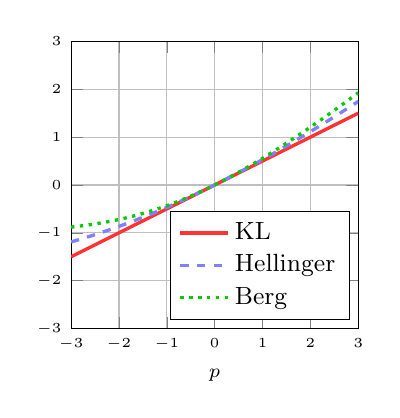
\begin{tikzpicture}
\iffalse
import sys
import numpy as np
from scipy.special import lambertw as W

p = np.linspace(-3, 3, 121)
a, b = 0.5, 1.5
eps, rho = 1, 1

# KL
kl = p * (rho / (rho + eps))

# Hellinger
hellinger = np.real(2 * eps * W((rho/eps) * np.exp((rho + p/2) / eps)) - 2*rho)

# Berg
berg = np.real(eps * W((rho/eps) * np.exp((rho + p) / eps)) - rho)

values = np.stack((p, kl, hellinger, berg)).T
np.savetxt(sys.stdout, values, fmt="%.3f")
\fi

    \pgfplotstableread{
    p balanced range tv
    -3.000 -1.500 -1.191 -0.880
    -2.950 -1.475 -1.176 -0.875
    -2.900 -1.450 -1.161 -0.869
    -2.850 -1.425 -1.147 -0.863
    -2.800 -1.400 -1.132 -0.857
    -2.750 -1.375 -1.116 -0.850
    -2.700 -1.350 -1.101 -0.844
    -2.650 -1.325 -1.085 -0.837
    -2.600 -1.300 -1.070 -0.830
    -2.550 -1.275 -1.054 -0.822
    -2.500 -1.250 -1.037 -0.815
    -2.450 -1.225 -1.021 -0.807
    -2.400 -1.200 -1.005 -0.798
    -2.350 -1.175 -0.988 -0.790
    -2.300 -1.150 -0.971 -0.781
    -2.250 -1.125 -0.954 -0.772
    -2.200 -1.100 -0.937 -0.762
    -2.150 -1.075 -0.919 -0.753
    -2.100 -1.050 -0.902 -0.743
    -2.050 -1.025 -0.884 -0.732
    -2.000 -1.000 -0.866 -0.722
    -1.950 -0.975 -0.848 -0.710
    -1.900 -0.950 -0.829 -0.699
    -1.850 -0.925 -0.811 -0.687
    -1.800 -0.900 -0.792 -0.675
    -1.750 -0.875 -0.773 -0.663
    -1.700 -0.850 -0.754 -0.650
    -1.650 -0.825 -0.735 -0.637
    -1.600 -0.800 -0.715 -0.623
    -1.550 -0.775 -0.695 -0.610
    -1.500 -0.750 -0.676 -0.595
    -1.450 -0.725 -0.656 -0.581
    -1.400 -0.700 -0.635 -0.566
    -1.350 -0.675 -0.615 -0.550
    -1.300 -0.650 -0.594 -0.535
    -1.250 -0.625 -0.574 -0.519
    -1.200 -0.600 -0.553 -0.502
    -1.150 -0.575 -0.532 -0.485
    -1.100 -0.550 -0.511 -0.468
    -1.050 -0.525 -0.489 -0.451
    -1.000 -0.500 -0.468 -0.433
    -0.950 -0.475 -0.446 -0.415
    -0.900 -0.450 -0.424 -0.396
    -0.850 -0.425 -0.402 -0.377
    -0.800 -0.400 -0.379 -0.358
    -0.750 -0.375 -0.357 -0.338
    -0.700 -0.350 -0.334 -0.318
    -0.650 -0.325 -0.311 -0.297
    -0.600 -0.300 -0.288 -0.276
    -0.550 -0.275 -0.265 -0.255
    -0.500 -0.250 -0.242 -0.234
    -0.450 -0.225 -0.219 -0.212
    -0.400 -0.200 -0.195 -0.190
    -0.350 -0.175 -0.171 -0.167
    -0.300 -0.150 -0.147 -0.144
    -0.250 -0.125 -0.123 -0.121
    -0.200 -0.100 -0.099 -0.097
    -0.150 -0.075 -0.074 -0.074
    -0.100 -0.050 -0.050 -0.049
    -0.050 -0.025 -0.025 -0.025
    0.000 0.000 0.000 0.000
    0.050 0.025 0.025 0.025
    0.100 0.050 0.050 0.051
    0.150 0.075 0.076 0.076
    0.200 0.100 0.101 0.102
    0.250 0.125 0.127 0.129
    0.300 0.150 0.153 0.155
    0.350 0.175 0.179 0.182
    0.400 0.200 0.205 0.210
    0.450 0.225 0.231 0.237
    0.500 0.250 0.258 0.265
    0.550 0.275 0.284 0.293
    0.600 0.300 0.311 0.321
    0.650 0.325 0.338 0.350
    0.700 0.350 0.365 0.379
    0.750 0.375 0.392 0.408
    0.800 0.400 0.419 0.437
    0.850 0.425 0.447 0.467
    0.900 0.450 0.474 0.497
    0.950 0.475 0.502 0.527
    1.000 0.500 0.530 0.557
    1.050 0.525 0.558 0.588
    1.100 0.550 0.586 0.619
    1.150 0.575 0.614 0.650
    1.200 0.600 0.643 0.681
    1.250 0.625 0.671 0.712
    1.300 0.650 0.700 0.744
    1.350 0.675 0.729 0.776
    1.400 0.700 0.758 0.808
    1.450 0.725 0.787 0.840
    1.500 0.750 0.816 0.873
    1.550 0.775 0.845 0.905
    1.600 0.800 0.875 0.938
    1.650 0.825 0.904 0.971
    1.700 0.850 0.934 1.005
    1.750 0.875 0.964 1.038
    1.800 0.900 0.993 1.072
    1.850 0.925 1.023 1.105
    1.900 0.950 1.054 1.139
    1.950 0.975 1.084 1.174
    2.000 1.000 1.114 1.208
    2.050 1.025 1.145 1.242
    2.100 1.050 1.175 1.277
    2.150 1.075 1.206 1.312
    2.200 1.100 1.237 1.347
    2.250 1.125 1.268 1.382
    2.300 1.150 1.299 1.417
    2.350 1.175 1.330 1.453
    2.400 1.200 1.362 1.488
    2.450 1.225 1.393 1.524
    2.500 1.250 1.424 1.560
    2.550 1.275 1.456 1.596
    2.600 1.300 1.488 1.632
    2.650 1.325 1.520 1.668
    2.700 1.350 1.552 1.705
    2.750 1.375 1.584 1.741
    2.800 1.400 1.616 1.778
    2.850 1.425 1.648 1.815
    2.900 1.450 1.680 1.852
    2.950 1.475 1.713 1.889
    3.000 1.500 1.745 1.926
    }\datatable
          
  
  \begin{axis}[width=.5\textwidth,grid=both,ymin=-3, ymax=3, xmin=-3, xmax=3,
      %title={\scriptsize We run NumPy, PyTorch and KeOps on a RTX 2080 Ti GPU.},
              xlabel={\scriptsize $p$}, 
              %ylabel={\scriptsize $-\aprox^\epsilon_{\phi^*}(-p)$}, 
              xtick={-3,-2,-1,0,1,2,3},
              %xticklabels={100,1k,10k,100k,1M},
              ytick={-3,-2,-1,0,1,2,3},
              %yticklabels={1\,ms,10\,ms,100\,ms,1\,s,10\,s},
              %xmode=log, ymode=log,
              legend pos = south east,
              %x post scale=1.7,
              grid=major,
            legend cell align={left},
            axis background/.style={fill=white},
            label style={font=\tiny},
            tick label style={font=\tiny},
            axis equal image,]
      \addplot[red!80, very thick,] table[x=p,y=balanced]  {\datatable};
      \addplot[blue!50, very thick, dashed] table[x=p,y=range]  {\datatable};
      \addplot[green!80!black, very thick, dotted] table[x=p,y=tv]  {\datatable};
      \addlegendentry{{\small KL}}
      \addlegendentry{{\small Hellinger}}
      \addlegendentry{{\small Berg}}
  \end{axis}
  \end{tikzpicture}}
	\caption{Display of the 1-Lipschitz operator $p \mapsto -\aprox{\phi^*}(-p)$ in the six major settings of Table~\ref{tab-entropies-aprox}, using $\epsilon=1$ and $\rho=1$.}
	\label{fig-aprox}
	%\end{figure}
	\vspace*{.7cm}
	
	\newcommand{\myfigE}[1]{\includegraphics[height=.14\linewidth]{images/compare_entropy/comparison_entropy_#1-c}}
	
	
	
	%\begin{figure}
	\centering
	\begin{tabular}{c@{\hspace{1mm}}c@{\hspace{1mm}}c@{\hspace{1mm}}}%
		\myfigE{reference} &
		\myfigE{Balanced} &
		\myfigE{KullbackLeibler} \\[-1mm]
		Inputs $(\al,\be)$ & $\iota_{(=)}$ & $10^{-1} * \KL$ \\[1mm]
		\myfigE{TotalVariation} &
		\myfigE{Range} &
		\myfigE{PowerEntropy} \\[-1mm]
		$10^{-1} * \TV$ & $\RG_{[0.7, 1.3]}$ & $10^{-1} * \text{Berg}$
	\end{tabular}
	\caption{Display of optimal marginals $(\textcolor{myred2}{\pi_1},\textcolor{myblue2}{\pi_2})$ depending on $\phi$. 
		The inputs $(\textcolor{myblue1}{\al},\textcolor{myred1}{\be})$ are 1D.
		Measures $(\textcolor{myblue1}{\al},\textcolor{myred1}{\be})$ and $(\textcolor{myred2}{\pi_1},\textcolor{myblue2}{\pi_2})$ are respectively plotted as dashed lines and filled colorings. 
		We use a regularization $\sqrt{\epsilon}=\sqrt{10^{-3}}$ on $[0,1]$.}
	\label{fig-comp-ent}
	%\end{figure}
	\vspace*{.7cm}
	
	\newcommand{\myfig}[1]{\includegraphics[width=.23\linewidth]{images/compare_reach/comparison_#1-c}}
	%\begin{figure}
	\centering
	\begin{tabular}{@{}c@{\hspace{1mm}}c@{\hspace{1mm}}c@{\hspace{1mm}}c@{\hspace{1mm}}c@{}}
		\rotatebox{90}{\small $\D_\phi=\rho\KL$} & \myfig{KullbackLeibler_reach001} & \myfig{KullbackLeibler_reach003} & \myfig{KullbackLeibler_reach013} & \myfig{KullbackLeibler_reach05} \\
		\rotatebox{90}{\small $\D_\phi=\rho\TV$\;\;} & \myfig{TotalVariation_reach001} & \myfig{TotalVariation_reach003} & \myfig{TotalVariation_reach013} & \myfig{TotalVariation_reach05} \\
		& $\rho=0.01$ & $\rho=0.03$ & $\rho=0.13$ & $\rho=0.5$
	\end{tabular}
	\caption{Display of marginals $(\textcolor{myred2}{\pi_1},\textcolor{myblue2}{\pi_2})$ depending on parameter $\rho$.
		We use the same inputs $(\textcolor{myblue1}{\al},\textcolor{myred1}{\be})$ from Figure~\ref{fig-comp-ent}. 
		First line corresponds to $\rho\KL$ and the second to $\rho\TV$.}
	\label{fig-impact-reach}
\end{minipage}
\end{figure}


\paragraph{Overview.}
%Figure~\ref{fig-aprox} displays $\aprox{\phi^*}$ for all aforementioned examples.
%We refer to Remark~\ref{rem-comment-sink} on its role of "dampening" balanced potentials.
%\begin{remark}\label{rem-comment-sink}
	We give an informal interpretation of Sinkhorn iterations for different divergences based on Proposition~\ref{prop-optimality-prox}, to illustrate the role of $\aprox{\phi^*}$.
	Optimality conditions have a compositional structure.
	Operators $(\Ss_\al,\Ss_\be)$ characterize optimal \emph{balanced} potentials as fixed points, and $\aprox{\phi^*}$ updates such fixed point by \emph{saturating} ($\D_\phi=\TV$) or \emph{dampening} ($\D_\phi=\KL$) dual potentials, see Figure~\ref{fig-aprox}.
	It indirectly impacts the plan via Equation~\eqref{eq-implicit-plan} by blocking or reducing transportation, see Figure~\ref{fig-impact-reach}.
%\end{remark}


Figure~\ref{fig-comp-ent} displays the impact of $\phi$ on the optimal plan $\pi$.
Here marginals $(\pi_1, \pi_2)$ are compared to the input marginals $(\al,\be)$.
Informally speaking, $\TV$ has 'sharp' marginals, i.e. it either transport s.t. $\pi_1(x)=\al(x)$ or destroys mass s.t. $\pi_1(x)=0$.
Marginals with $\KL$ are 'smooth' in the sense that it progressively transitions between transportation and destruction as $\C(x,y)$ increases.
Marginals for $\RG_{[a,b]}$ are less interpretable due to the box constraint, but we see that $\tfrac{\d\pi_1}{\d\al}\in\{a,b\}$.
The result of Berg entropy is similar to $\KL$, probably because they are both power entropies.
%
%\todo{Est-ce qu'on devrait supprimer ce paragraphe non mathématique ?}
%One sees that the marginals for $\KL$ have full support and that the density dampens as the distance between supports increases. For $\TV$ the density either matches the input or cancels out. The Range entropy is less intuitive due to the box constraint, the ratio of the density being equal to either one bound of the box or the other.
%The Berg entropy is represented here as an instance of the family of power entropies which includes the $\KL$, whence their similar behaviours.


Figure~\ref{fig-impact-reach} shows the impact of the parameter $\rho$ on $(\pi_1,\pi_2)$ (see Remark~\ref{rem-param-rho}). 
It illustrates that $\rho$ acts as a characteristic radius beyond which it is preferable to destroy mass than transport it. 
This phenomenon is sharp in the case of $\TV$ (it is known when $\epsilon=0$ that $\spt(\pi)\subset\{(x,y), \C(x,y)\leq 2\rho\}$) while there is a smooth dampening as $\C$ increases for $\KL$.


%
%\newcommand{\myfig}[1]{\includegraphics[width=.23\linewidth]{images/compare_reach/comparison_#1-c}}
%\begin{figure}
%	\centering
%	\begin{tabular}{@{}c@{\hspace{1mm}}c@{\hspace{1mm}}c@{\hspace{1mm}}c@{\hspace{1mm}}c@{}}
%		\rotatebox{90}{\small $\D_\phi=\rho\KL$} & \myfig{KullbackLeibler_reach001} & \myfig{KullbackLeibler_reach003} & \myfig{KullbackLeibler_reach013} & \myfig{KullbackLeibler_reach05} \\
%		\rotatebox{90}{\small $\D_\phi=\rho\TV$\;\;} & \myfig{TotalVariation_reach001} & \myfig{TotalVariation_reach003} & \myfig{TotalVariation_reach013} & \myfig{TotalVariation_reach05} \\
%		& $\rho=0.1$ & $\rho=0.03$ & $\rho=0.13$ & $\rho=0.5$
%	\end{tabular}
%	\caption{Display of the impact of the reach parameter $\rho$ on the marginals $(\textcolor{myred2}{\pi_1},\textcolor{myblue2}{\pi_2})$ given the same inputs $(\textcolor{myblue1}{\al},\textcolor{myred1}{\be})$ from Figure~\ref{fig-comp-ent}. First line corresponds to $\rho\KL$ and the second to $\rho\TV$.}
%	\label{fig-impact-reach}
%\end{figure}


\begin{table}
	\centering
	\def\arraystretch{1.2}
	\begin{adjustbox}{center}
		\begin{tabular}{|c@{}c@{\hspace{2mm}}c@{}c|}
			\hline
			Setting & Parameters & $\phi(p)$ & $-\aprox{\phi^*}(-p)$\\
			\hline
			Balanced & None & $0$ if $p=1$, $+\infty$ otherwise & $p$ \\
			Range & $0 \leq a \leq 1 \leq b$ & $0$ if $p \in [a, b]$, $+\infty$ otherwise &
			$\text{Soft-Thresh}_{\epsilon \log a}^{\epsilon \log b}(p)$ \\
			TV & $\rho > 0$ & $\rho\, |p-1|$ & $\text{Clamp}_{[-\rho, +\rho]}(p)$  \\
			KL & $\rho > 0$ & $\rho\, (p \log p - p + 1)$ & $\tfrac{\rho}{\rho+\epsilon}\, p$ \\
			Hellinger & $\rho > 0$ & $4 \rho\, (1 + (p-1)/2 - \sqrt{p})$ &  $2 \epsilon W(\tfrac{\rho}{\epsilon} \exp(\tfrac{\rho+p/2}{\epsilon})) - 2\rho $ \\
			Berg & $\rho > 0$ & $\rho\, (p - 1 - \log p)$ & $\epsilon W(\tfrac{\rho}{\epsilon} \exp(\tfrac{\rho+p}{\epsilon})) - \rho$ \\
			\hline
		\end{tabular}
	\end{adjustbox}
	\caption{Summary of the information that is required to implement
		the generalized Sinkhorn algorithm in six common settings.
	}
	\label{tab-entropies-aprox}
\end{table}





%%%%%%%%%%%%%%%%%%%%%%%%%%%%%%
\subsection{Convergence analysis and compactness of potentials}
\label{sec-convergence}

For discrete measures, alternate maximization is known to converge to maximizers for smooth problems~\cite{tseng2001convergence}, 
%
but convergence speeds known in the litterature depend on the number of samples.
Until now, there was no proof for general (continuous) measures.
%
In this section, we work over the \emph{infinite dimensional} space $\Mmp(\Xx)$ to overcome these limitations.
We prove linear convergence of the unbalanced Sinkhorn algoritm in full generality in Theorem~\ref{thm-cv-sink-compact} which is the main result of this section.


%%%%%%%%%%%%%%%%%%%%%%%%%%%%%%%%%%%%%%%%%%%%%%%%%%%%%%%%%%%%
\subsubsection{General convergence result}

Theorem~\ref{thm-cv-sink-compact} states convergence of Sinkhorn iterates, provided they remain in a compact subset of $\Cc(\Xx)^2$.
%
We then prove that this compactness hypothesis holds in a variety of settings, including Section~\ref{sec-exmp-f-div}.
A first setting studied in Section~\ref{subsubsec-convergence-compact} assumes $\phi^*$ is strictly convex, and holds in wide generality.
%A first case studied in Section~\ref{subsubsec-convergence-compact} is the one of strictly convex entropies that can be studied in full generality. 
The settings of balanced OT, TV and Range are convex but not strictly. They are treated separately in Section~\ref{sec-compact-balanced-tv-range}.

\begin{theorem}[The Sinkhorn algorithm solves the $\OTb$ problem]\label{thm-cv-sink-compact}
If the cost $\C$ is $\gamma$-Lipschitz, and if the dual program~\eqref{eq-dual-unb} can be restricted to a compact subset of $\Cc(\Xx)^2$, then there exists an optimal pair of dual potentials and the Sinkhorn algorithm converges towards a pair of optimal potentials.
%
In particular we have convergence for all settings of Section~\ref{sec-exmp-f-div}.
\end{theorem}

\begin{proof}
Consider a sequence $(\f_n,\g_n)_n$ approaching $\OT(\al,\be)=\sup\Ff$. 
Compactness in $\Cc(\Xx)$ allows to extract $(\f_{n_k},\g_{n_k})\rightarrow(\f,\g)$, where $(\f,\g)\in\Cc(\Xx)^2$ are optimal, i.e. $\OT(\al,\be)=\Ff(\f,\g)$.

Now write $(\f_t,\g_t)$ the Sinkhorn iterates~\eqref{eq-sinkhorn-iter-1} for some $\f_0\in\Cc(\Xx)$.
Iterates $(\f_t,\g_t)$ are $\gamma$-Lipschitz (Proposition~\ref{lem-smin-cost-regular}), thus equicontinuous on $\Xx$. 
Furthermore, non-expansivity of $\Aa\Ss$ (Propositions~\ref{lem-smin-lipschitz-func} and~\ref{prop-nonexp}) implies $\norm{\f_t - \f}_\infty\leq\norm{\f_{0} - \f}_\infty$.
Since $\f\in\Cc(\Xx)$ and $\Xx$ compact, then $\norm{\f}_\infty < \infty$. 
Thus $\norm{\f_t}_\infty \leq\norm{\f_{0} - \f}_\infty + \norm{\f}_\infty$.

Ascoli-Arzela theorem holds and Sinkhorn iterates $(\f_t,\g_t)_t$ are a compact sequence in $\Cc(\Xx)$.
Take any subsequence $\f_{t_k}\rightarrow \f_*$, and $\eta >0$. There exists $k$ such that $\norm{\f_{k} - \f_*}_\infty < \eta$. 
Non-expansivity of $\Aa\Ss$ implies again that $\forall t\geq k,\, \norm{\f_{t} - \f_*}_\infty\leq\norm{\f_{k} - \f_*}_\infty < \eta$.
The same fact holds for $(\g_t)$
This inequality is the definition of the convergence of $(\f_t)$.
Thus any subsequence verifies $\f_{t_k}\rightarrow\f_*$ and then $\f_t\rightarrow\f_*$. 
Thus Sinkhorn iterates converge towards $(\f_*,\g_*)$ and are fixed point of the Sinkhorn maps.
Thus they are optimal (Proposition~\ref{prop-cns-optimality}).

Thanks to Lemmas~(\ref{lem-compact-dual},\ref{lem-compact-balanced},\ref{lem-compact-tv},\ref{lem-compact-range}), we can restrict Problem~\eqref{eq-dual-unb} to a compact set, hence the convergence for all settings of Section~\ref{sec-exmp-f-div}.
\end{proof}

Theorem~\ref{thm-cv-sink-compact} reduces proofs of \emph{convergence} to proofs of \emph{compactness} of the sequence $(\f_n,\g_n)$. 
We detail these results in Sections~\ref{subsubsec-convergence-compact} and~\ref{sec-compact-balanced-tv-range}.
We give before a sufficient condition of convergence when $\aprox{\phi^*}$ is contractive.
It holds for $\KL$ and some Power entropies (see Proposition~\ref{prop-aprox-power-ent}).
%but first give a sufficient condition on the convergence of the Sinkhorn algorithm when the aprox operator is contractive. All families of strictly convex entropy functions shown in Section~\ref{sec-exmp-f-div} induce proximity operators that are contractions on compact sets, and can thus benefit from this direct proof.

\begin{proposition}\label{prop-contractive-sink}
If $\aprox{\phi^*}$ is a contraction on compact sets w.r.t.~$\norm{\cdot}_\infty$ and if $\C$ is $\gamma$-Lipschitz, then the Sinkhorn algorithm converges linearly towards a unique fixed point w.r.t $\norm{\cdot}_\infty$.
\end{proposition}

\begin{proof}
The Softmin is non-expansive (Lemma~\ref{lem-smin-lipschitz-func}) and Lemma~\ref{lem-smin-cost-regular} gives the continuity of $\Ss_\al(\f)$ and $\Ss_\be(g)$, which are bounded on compact sets. Thus composing with $\aprox{\phi^*}$ gives a contractive mapping with respect to $\norm{.}_\infty$.
\end{proof}

\begin{remark}\label{rem-cv-balanced-sink}
	A similar contraction theorem holds for \emph{balanced} OT.
	The Birkhoff-Hopf theorem from non-linear Perron-Frobenius theory~\cite{lemmens2012nonlinear} states that $(\Ss_\al,\Ss_\be)$ are contractive w.r.t. the Hilbert pseudo-norm.
\end{remark}
%Note that .
%In this case, the Birkhoff theorem of non-linear Perron Frobenius theory allows us to show that the Softmin is contractive with respect to the Hilbert metric ~\cite{lemmens2012nonlinear}.


%%%%%%%%%%%%%%%%%%%%%%%%%%%%%%%%%%%%%%%%%%%%%%%%%%%%%%%%%%%%
\subsubsection{Lemmas on compactness of potentials}
\label{subsubsec-lemma-factor-compact}

This section reduces the proof of compactness in two parts thanks to the structure of $\Ff(\f,\g)$.
Lemma~\ref{lem-uniq-tensor-sum} below states $(\f,\g)$ are optimal up to translations $(\f+\lambda,\g-\lambda)$ for $\lambda\in\R$.
This invariance allows to assume $\f(x_0)=0$ for some $x_0\in\Xx$, and to build a compact set in Lemma~\ref{lem-compact-anchor}.
It then remains to prove that admissible translations $\lambda$ lie in a compact set, which is treated in Sections~\ref{subsubsec-convergence-compact} and~\ref{sec-compact-balanced-tv-range}.

\begin{lemma}[Uniqueness of the optimal dual pair]\label{lem-uniq-tensor-sum}
For any $(\al,\be)\in\Mmpp(\Xx)$, there is uniqueness of optimal potentials $(\f,\g)$ for the dual program~\eqref{eq-dual-unb} in the following sense: if there are two optimal solutions $(\f_1,\g_1)$ and $(\f_2,\g_2)$ then $\f_1\oplus\g_1 = \f_2\oplus\g_2$, $\alpha \otimes \beta$-a.e.. Thus, given optimal potentials $\f\oplus\g$, all other optimal ones can only be $\alpha \otimes \beta$-a.e. of the form $(\f + \lambda, \g-\lambda)$ for some $\lambda\in\R$.
\end{lemma}
%\begin{proof}
% Denote the dual functional~\eqref{eq-dual-unb} as $\mathcal{F}$ and assume  the existence of two couples of dual potentials $(f_1,g_1)$ and $(f_2,g_2)$ such that $ \mathcal{F}(f_1,g_1) = \mathcal{F}(f_2,g_2)$. Due to the optimality of potentials and the joint convexity of $\Ff$ we have that
% $\mathcal{F}(t f_1 + (1-t) f_2, t g_1 + (1-t) g_2) = t \mathcal{F}(f_1,g_1) + (1-t) \mathcal{F}(f_2,g_2)$.
%Because the function $h\mapsto -\dotp{\al\otimes\be}{e^{(h -\C)/\epsilon} }$ is strictly concave on the support of $\al\otimes\be$, the previous equality imposes
%\begin{multline}
% \dotp{\al\otimes\be}{e^{(t f_1 \oplus g_1 + (1-t) f_2 \oplus g_2 -\C)/\epsilon} } \\=  \dotp{\al\otimes\be}{te^{( f_1 \oplus g_1  -\C)/\epsilon}  + (1-t) e^{( f_2 \oplus g_2 -\C)/\epsilon} }\,,
%\end{multline}
%Again due to the strict convexity and because we integrate continuous functions against positive measures, we deduce a pointwise equality that $\alpha \otimes \beta$ a.e., one has
%$t (f_1(x)+g_1(y)) + (1-t)(f_2(x) + g_2(y)) = f_1(x)+g_1(y) = f_2(x) + g_2(y)$,
%which implies $f_1 \oplus g_1 = f_2 \oplus g_2$, $\alpha \otimes \beta$ a.e.
%\end{proof}
\begin{proof}
	Write $(\f_1,\g_1)$ and $(\f_2,\g_2)$ two optimal pairs for~\eqref{eq-dual-unb}, and define $\f_t=t\f_1 + (1-t)\f_2$ and $\g_t=t\g_1 + (1-t)\g_2$ with $t\in[0,1]$. Write
	\begin{align*}
		a_1 &= \dotp{\al}{-\phi^*(-\f_t)} + \dotp{\be}{-\phi^*(-\g_t)},\\
		a_2 &= \dotp{\al}{-t\phi^*(-\f_1) - (1-t)\phi^*(-\f_2)} + \dotp{\be}{-t\phi^*(-\g_1) - (1-t)\phi^*(-\g_2)},\\
		b_1 &= -\epsilon\dotp{\al\otimes\be}{e^{(\f_t\oplus\g_t-\C) / \epsilon} - 1},\\
		b_2 &= -\epsilon\dotp{\al\otimes\be}{t e^{(\f_1\oplus\g_1-\C) / \epsilon} + (1-t)e^{(\f_2\oplus\g_2-\C) / \epsilon} - 1}.
	\end{align*}
	By optimality and convexity of the problem one has $a_1 + b_1 = a_2 + b_2$ as well as $a_1\geq a_2$ and $b_1\geq b_2$, thus necessarily $a_1=a_2$ and $b_1=b_2$. In particular the equality $b_1=b_2$ is an integral against a positive measure whose integrand verifies pointwise $e^{(\f_t(x)\oplus\g_t(y)-\C) / \epsilon}\leq te^{(\f_1(x)\oplus\g_1(y)-\C) / \epsilon} + (1-t)e^{(\f_2(x)\oplus\g_2(y)-\C) / \epsilon}$, thus the inequaliy becomes a pointwise equality holding $\al\otimes\be$-a.e. Eventually, the strict convexity of the exponential yields $\al\otimes\be$-a.e. that $t (f_1(x)+g_1(y)) + (1-t)(f_2(x) + g_2(y)) = f_1(x)+g_1(y) = f_2(x) + g_2(y)$.
\end{proof}

We warn that not all $\lambda$ yield an optimal pair.
There exists a unique $\lambda$ for strictly convex $\phi^*$, while any $\lambda\in\R$ is optimal for balanced OT.
%The above lemma asserts that the possibly optimal potentials of the dual program are necessarily of the form $(\f + \lambda, \g-\lambda)$ -- but not all $\lambda$ yield an optimal pair. We prove in the following lemma that we can restrict the dual program to a set of functions which will be proved to be compact. It then remains to prove compactness with respect to $\lambda$, which is detailed in Sections~\ref{subsubsec-convergence-compact} and~\ref{sec-compact-balanced-tv-range}.


\begin{lemma}[Compact Anchoring of $(\f,\g)$]\label{lem-compact-anchor}
	Assume $\C$ is $\gamma$-Lipschitz, and define 
	$\Pp_{x_o} \eqdef \{ (\f,\g)\in\Aa\Ss_\be(\Cc(\Xx))\times\Aa\Ss_\al(\Cc(\Xx)),\, \f(x_0) = 0,\,\exists M\in\R,\, \norm{\f\oplus\g}_\infty \leq M \}$ 
	for some $x_0\in\Xx$.
	Then one can restrict the dual~\eqref{eq-dual-unb} as a supremum over $\Pp_{x_o}+\R \eqdef\{(\f + \lambda,\g-\lambda),\, (\f,\g)\in\Pp_{x_0},\, \lambda\in\R\}$.
	Furtermore the set $\Pp_{x_o}$ is relatively compact in $\Cc(\Xx)$.
\end{lemma}
\begin{proof}
	Optimality of $(\f,\g)$ is equivalent to have $(\f,\g)=(\Aa\Ss_\be(\g), \Aa\Ss_\al(\f))$ (Proposition~\ref{prop-cns-optimality}), hence the restriction to $\Aa\Ss_\be(\Cc(\Xx))\times\Aa\Ss_\al(\Cc(\Xx))$.
	Such potentials are $\gamma$-Lipschitz (Lemma~\ref{lem-smin-cost-regular}).
	
	We show that in $\Aa\Ss_\be(\Cc(\Xx))\times\Aa\Ss_\al(\Cc(\Xx))$, there exists $\tilde{M}$ s.t. $\norm{\f\oplus\g}_\infty \leq \tilde{M}$.
	Consider a sequence $(\f_n,\g_n)_n$ such that $\norm{\f_n\oplus\g_n}_\infty\rightarrow+\infty$. 
	We have $(\f_n,\g_n)\in\Cc(\Xx)$ with $\Xx$ compact, thus $\exists(x_n,y_n)\in\Xx^2,\,\norm{\f_n\oplus\g_n}_\infty=(\f_n\oplus\g_n)(x_n,y_n)$. 
	We have $(\f_n\oplus\g_n)(x_n,y_n)\rightarrow+\infty$. 
	Since $(\f_n,\g_n)$ are $\gamma$-Lipschitz, $\forall(x,y)\in\Xx^2,\, |(\f_n\oplus\g_n)(x_n,y_n) - (\f_n\oplus\g_n)(x,y)|\leq 2\gamma \text{diam}(\Xx)$, thus $\norm{\f_n\oplus\g_n}_\infty - 2\gamma \text{diam}(\Xx) \leq (\f_n\oplus\g_n)(x,y)$. 
	When $(x,y)\in\spt(\al)\times\spt(\be))$, $(\f_n\oplus\g_n)(x,y)\rightarrow+\infty$ and $\Ff(\f_n,\g_n)\rightarrow-\infty$.
	Similarly, if $(\f_n\oplus\g_n)(x_n,y_n)\rightarrow-\infty$ then $\Ff(\f_n,\g_n)\rightarrow-\infty$. 
	Hence we have $\norm{\f\oplus\g}_\infty \leq \tilde{M}$.
	
	Assume $\norm{\f\oplus\g}_\infty \leq \tilde{M}$.
	Potentials $(\f+\lambda,\g-\lambda)$ with $\lambda\in\R$ have the same bound. 
	Thus w.l.o.g. $\f(x_0)=0$ for some $x_0\in\Xx$. 
	Since $\f$ is $\gamma$-Lipschitz, we have $\norm{\f}_\infty \leq\gamma \text{diam}(\Xx)$ because $\f(x_0)=0$.
	Thus $\norm{\g}_\infty \leq \norm{\f} + \norm{\f\oplus\g}_\infty \leq \gamma \text{diam}(\Xx) + \tilde{M} = M.$
	Thus potentials in $E$ satisfy all properties.
	
	In $\Pp_{x_0}$ potentials are uniformly equicontinuous because $\norm{\f}_\infty,\norm{\g}\leq M$.
	Ascoli-Arzela theorem holds, and $\Pp_{x_0}$ is relatively compact in $\Cc(\Xx)$.
\end{proof}

%\begin{lemma}[Anchoring of the dual potentials]\label{lem-restrict-pot}
%If the cost $\C$ is $\gamma$-Lipschitz, the dual program~\eqref{eq-dual-unb} can be restricted to a subset of functions of $\Tt_\be(\Cc(\Xx))\times\Tt_\al(\Cc(\Xx))$ of the form $(\f+\lambda,\g-\lambda)$ with $\lambda\in\R$, such that $\f(x_0)=0$ for some $x_0\in\Xx$ and such that $(\f,\g)$ satisfies $\norm{\f}_\infty \leq M$ and $\norm{\g}_\infty \leq M$ for some finite $M\in\R_+$.
%\end{lemma}
%\begin{proof}
%Optimality of potentials is equivalent to be a fixed point of the Sinkhorn mapping (Proposition~\ref{prop-cns-optimality}), thus we can restrict to potentials in $E = \Tt_\be(\Cc(\Xx))\times\Tt_\al(\Cc(\Xx))$. Such potentials are $\gamma$-Lipschitz (Lemma~\ref{lem-smin-cost-regular}).
%
%We show that in $E$, $\norm{\f\oplus\g}_\infty \leq \tilde{M}$.
%Consider a sequence $(\f_n,\g_n)_n$ such that $\norm{\f\oplus\g}_\infty\rightarrow+\infty$. 
%We have $(\f_n,\g_n)\in\Cc(\Xx)$ with $\Xx$ compact, thus $\exists(x_n,y_n)\in\Xx^2,\,\norm{\f_n\oplus\g_n}_\infty=(\f_n\oplus\g_n)(x_n,y_n)$. 
%We have $(\f_n\oplus\g_n)(x_n,y_n)\rightarrow+\infty$. 
%Since $(\f_n,\g_n)$ are $\gamma$-Lipschitz, $\forall(x,y)\in\Xx^2,\, |(\f_n\oplus\g_n)(x_n,y_n) - (\f_n\oplus\g_n)(x,y)|\leq 2\gamma \text{diam}(\Xx)$, thus $\norm{\f_n\oplus\g_n}_\infty - 2\gamma \text{diam}(\Xx) \leq (\f_n\oplus\g_n)(x,y)$. 
%When $(x,y)\in\spt(\al)\times\spt(\be))$, $(\f_n\oplus\g_n)(x,y)\rightarrow+\infty$ and $\Ff(\f_n,\g_n)\rightarrow-\infty$.
%Similarly, if $(\f_n\oplus\g_n)(x_n,y_n)\rightarrow-\infty$ then $\Ff(\f_n,\g_n)\rightarrow-\infty$. 
%Hence we have $\norm{\f\oplus\g}_\infty \leq \tilde{M}$.
%
%Assume $\norm{\f\oplus\g}_\infty \leq \tilde{M}$.
%Potentials $(\f+\lambda,\g-\lambda)$ with $\lambda\in\R$ have the same bound. 
%Thus w.l.o.g. $\f(x_0)=0$ for some $x_0\in\Xx$. 
%Since $\f$ is $\gamma$-Lipschitz, we have $\norm{\f}_\infty \leq\gamma \text{diam}(\Xx)$ because $\f(x_0)=0$.
%Thus $\norm{\g}_\infty \leq \norm{\f} + \norm{\f\oplus\g}_\infty \leq \gamma \text{diam}(\Xx) + \tilde{M} = M.$
%Thus potentials in $E$ satisfy all properties.
%
%In $\Pp_{x_0}$ potentials are uniformly equicontinuous.
%Ascoli-Arzela theorem holds, and $\Pp_{x_0}$ is relatively compact in $\Cc(\Xx)$.
%\end{proof}
%
%In what follows we always consider such set of functions, because it is compact as stated below. 
%%The next lemma asserts that the set of potentials with an anchor point is compact. Thus it remains to prove that the set of such translated potentials that yields an optimal pair of potentials is compact.
%
%\begin{lemma}[Relative compactness of sets of anchored potentials]\label{lem-compact-anchor}
%Let $\C$ be a $\gamma$-lipschitz cost function. For any $(\al,\be)\in\Mmpp(\Xx)$ the sets
% $\Pp_{x_o} = \{ (\f,\g)\in\Tt_\be(\Cc(\Xx))\times\Tt_\al(\Cc(\Xx)),\, \f(x_0) = 0,\, \norm{\f\oplus\g}_\infty \leq M \} $
% are relatively compact in $\Cc(\Xx)$.
%\end{lemma}
%\begin{proof}
%Reusing the above proof of Lemma~\ref{lem-restrict-pot}, we get that for any $(\f,\g)\in\Pp_{x_0}$, the potentials $(\f,\g)$ are $\gamma$-Lipschitz and verify $\norm{\f}_\infty \leq \tilde{M}$ and $\norm{\g}_\infty \leq  \tilde{M}$. Thus $\f$ and $\g$ are both uniformly equicontinuous. The Ascoli-Arzela theorem applies, which gives that the set $\Pp_{x_0}$ is relatively compact in $\Cc(\Xx)$.
%\end{proof}


%%%%%%%%%%%%%%%%%%%%%%%%%%%%%%%%%%%%%%%%%%%%%%%%%%%%%%%%%%%%
\subsubsection{Compactness for strictly convex entropies}
\label{subsubsec-convergence-compact}

We prove compactness of potentials under two fairly general assumptions.

\begin{assumption}\label{as:1}
  The function $\phi^*$ is strictly convex.
\end{assumption}
\begin{assumption}\label{as:2}
  There exists a sequence $(x_n)_n \subset \text{\upshape dom}(\phi^*)$ and $s_n\in\partial\phi^*(x_n)$ such that $s_n$ converges either to zero or $+\infty$. 
\end{assumption}
The cases of $\KL$ and Power entropies mentioned Section~\ref{sec-exmp-f-div} satisfy those assumptions.
%The Kullback-Leibler and the power-entropies are the divergences mentioned in Section~\ref{sec-exmp-f-div} which verify both  assumptions.
%
%This property is fundamental to ensure existence and uniqueness of potentials, and prove the weak* differentiability of our optimal transport loss.
This setting ensures existence and uniqueness of optimal $(\f,\g)$, the latter being key for weak* differentiability of $\OTb$ and $\Sb$.
%
%We detail the need for those assumptions in Example~\ref{exmp-range2}, at the end of this Section.

\begin{lemma}[Restriction of the dual $\OTb$ problem to a compact set]\label{lem-compact-dual}
Let $\C$ be a $\gamma$-lipschitz cost function. Under Assumption~\ref{as:2}, the dual problem~\eqref{eq-dual-unb} can be restricted to a supremum over the compact set $\overline{\Pp_{x_0} + I}$ where
\begin{align*}
  \Pp_{x_0} + I = \{ (\f+\lambda,\g-\lambda),\, (\f,\g)\in\Pp_{x_0}, \lambda\in I \}
\end{align*}
with $I$ being a compact set. Furthermore, the compact interval $I$ only depends on $(m(\al),m(\be))$ in a neighborhood of $(\al,\be)$ and this dependency is continuous.
\end{lemma}

\begin{proof}
Lemma~\ref{lem-compact-anchor} applies, thus we consider potentials $(\f+\lambda,\g-\lambda)$ with $(\f,\g)\in\Pp_{x_0}$ (relatively compact) and $\lambda\in\R$.
It remains to prove that the dual program~\eqref{eq-dual-unb} is coercive w.r.t. $\lambda$.

Since $\phi^*$ is convex one has for any $q$ such that $-q\in\text{dom}(\phi^*)$ and $s\in\partial\phi^*(-q)$
\begin{align*}
  \dotp{\al}{-\phi^*(-\f-\lambda)} &\leq \dotp{\al}{-\phi^*(-q) +s(\f + \lambda-q)} \\
  &\leq m(\al) \big(  -\phi^*(-q) +s(\norm{\f}_\infty + \lambda-q) \big).
\end{align*}
From this and the similar inequality for $\be$, we deduce for any $(-q,-\tilde{q})\in\text{dom}(\phi^*)$ and $(s,\tilde{s})\in\partial\phi^*(-q)\times\partial\phi^*(-\tilde{q})$ that
%\begin{align*}
%  \dotp{\al}{-\phi^*(-\f - \lambda)} &+ \dotp{\be}{-\phi^*(-\g + \lambda)}\\
%  &\leq \big[m(\al)s - m(\be)\tilde{s}\big]\lambda \eqdef R(s, \tilde{s})\lambda\\
%   &\begin{array}{@{}l}+ m(\al)\big(-\phi^*(-q) + s(\norm{\f}_\infty -q) \big)\\ + m(\be)\big(-\phi^*(-\tilde{q}) + \tilde{s}(\norm{\g}_\infty -\tilde{q}) \big)\end{array} \Big\}\eqdef K.
%\end{align*}
\begin{align*}
\Ff(\f+\lambda,\g-\lambda)=\dotp{\al}{-\phi^*(-\f - \lambda)} &+ \dotp{\be}{-\phi^*(-\g + \lambda)}\leq  R(s, \tilde{s})\lambda + K,%(m(\al), m(\be), \norm{\f}_\infty, \norm{\g}_\infty, q, \tilde{q}, s, \tilde{s}),
\end{align*}
where $R(s, \tilde{s})\eqdef m(\al)s - m(\be)\tilde{s}$ and
\begin{align*}
	K \eqdef m(\al)\big(-\phi^*(-q) + s(\norm{\f}_\infty -q) \big)+ m(\be)\big(-\phi^*(-\tilde{q}) + \tilde{s}(\norm{\g}_\infty -\tilde{q}) \big).
\end{align*}
To be coercive in $\lambda$, we need to find points $(q_1,\tilde{q}_1)\in\text{dom}(\phi^*)^2$, $(s_1, \tilde{s}_1)\in\partial\phi^*(q_1)\times\partial\phi^*(\tilde{q}_1)$ and $(q_2,\tilde{q}_2)\in\text{dom}(\phi^*)^2$, $(s_2, \tilde{s}_2)\in\partial\phi^*(q_2)\times\partial\phi^*(\tilde{q}_2)$ such that $K<+\infty$ (it holds on $\text{dom}(\phi^*)$), such that $R(s_1,\tilde{s}_1) > 0$ and $R(s_2,\tilde{s}_2) < 0$. 
Assumption~\ref{as:2} proves it. 
We have $\partial\phi^*\subset\R_+$. 
If  $\exists s_n\in\partial\phi^*(x_n)$ with $s_n\rightarrow 0$, take $q_1\in\text{dom}(\phi^*)$ and $\tilde{q}_1=x_n$.
There exists $n_0$, such that $s_n$ is small enough for $n\geq n_0$ and $R(s_1, s_n)>0$. 
Similarly we find some $R(s_2, \tilde{s}_2)<0$. 
The same approach holds for $\partial\phi^*(x_n)\rightarrow +\infty$. 
Thus $\Ff(\f+\lambda,\g-\lambda)\rightarrow-\infty$ when $\lambda\rightarrow\pm\infty$ by taking either $R<0$ or $R>0$.

Note that $(R,K)$ depends continuously on $(m(\al),m(\be))$. Thus, on a neighbourhood of $(\al,\be)$, one still has $R(s_1, \tilde{s}_1) > 0$, $R(s_2, \tilde{s}_2) < 0$ and $|K|<\infty$.

Coercivity holds and $\lambda$ is in a compact interval $I$ that is constant in a neighborhood of $(\al,\be)$. 
Thus the optimal potentials can be taken in a set $\Pp_{x_0}+I$. 
The potentials inside this set remain equicontinuous and uniformly bounded. 
The Ascoli-Arzelà theorem applies and $\Pp_{x_0}+I$ is relatively compact in $\Cc(\Xx)$.
\end{proof}

Lemma~\ref{lem-compact-dual} and Assumptions~\ref{as:1} ensure existence and uniqueness of optimal $(\f,\g)$.
We now prove $(\f,\g)$ depend continuously in $(\al,\be)$, which is key for the weak* regularity of $\OTb$ studied in Section~\ref{sec-ot-prop}. 
%Note that under Assumption~\ref{as:1}, the dual~\eqref{eq-dual-unb} is strictly convex in $(\f,\g)$: there is uniqueness of the optimal pair.

\begin{proposition}[The dual potentials vary continuously with the input measures]
\label{prop-uniform-conv}
Let $\C$ be a $\gamma$-lipschitz cost function.
Let $\al_n \rightharpoonup \al$ and
$\be_n \rightharpoonup \be$ be weakly converging
sequences of measures in $\Mmpp(\Xx)$.
Write $(\f_n,\g_n)$ the (unique) sequence of optimal
potentials for $\OTb(\al_n,\be_n)$.

Under Assumptions~\ref{as:1} and \ref{as:2}, $\f_n$ and $\g_n$ converge uniformly towards the
unique pair of optimal potentials $(\f,\g)$ for $\OTb(\al,\be)$:
\begin{align*}
\big( \al_n \rightharpoonup \al, \,
\be_n \rightharpoonup \be
\big)\Longrightarrow
\big( \f_n \xrightarrow{\|\cdot\|_\infty} \f, \,
\g_n \xrightarrow{\|\cdot\|_\infty} \g
\big).
\end{align*}
\end{proposition}

\begin{proof}
  Thanks to Theorem~\ref{thm-cv-sink-compact}, for all $(\al_n,\be_n)$, $\exists !(\f_n,\g_n)$ optimal in $\OTb(\al_n,\be_n)$. 
  Applying Lemma~\ref{lem-compact-dual}, we assume $(\f_n,\g_n)\in\Pp_{x_0}+I_n$.
  The interval $I_n$ depends continuously in $(m(\al_n),m(\be_n))$ in a neighborhood of $(\al_n,\be_n)$. 
  Since $(\al_n,\be_n)\rightharpoonup(\al,\be)$ with $m(\al),m(\be)>0$,
  there exists $(-q_i, -\tilde{q}_i)\in\text{dom}(\phi^*)^2$, $(s_i,\tilde{s}_i)\in\partial\phi^*(-q_i)\times\partial\phi^*(-\tilde{q}_i)$, $\eta >0$ and $n_0$ such that for all $n \geq n_0$
\begin{gather*}
  0 < m(\al) -\eta < m(\al_n) < m(\al) +\eta \; \text{and} \; 0 < m(\be) -\eta < m(\be_n) < m(\be) +\eta\\
  \Rightarrow R_+ \eqdef (m(\al)-\eta)s_1 - (m(\be)+\eta)\tilde{s}_1 < R(s_1,\tilde{s}_1)<0,\\
   \Rightarrow R_- \eqdef (m(\al)+\eta)s_2 - (m(\be)-\eta)\tilde{s}_2 > R(s_1,\tilde{s}_1)>0,
\end{gather*}
where $R$ is defined in the proof of Lemma~\ref{lem-compact-dual}. 
Again, Assumption~\ref{as:2} guarantees that we find points in $\text{dom}(\phi^*)$, independent of $n$, such that $\forall n \geq n_0$, $R_+ <0$ and $R_- >0$. 
We then build a compact subset $\Pp_{x_0}+I$ with $I$ compact and independent of $n$ such that for all $n$, $(\f_n,\g_n)\in\Pp_{x_0}+I$.
Ascoli-Arzelà theorem holds.
   One  extracts a subsequence $(\f_{n_k},\g_{n_k})\rightarrow(\f,\g)$, where $(\f,\g)$ are unique optimal in $\OTb(\al,\be)$. 
   All subsequences converge to the same limit due to uniqueness of optimal potentials. 
   Hence we get $(\f_n,\g_n)\rightarrow(\f,\g)$.
\end{proof}

%%%%%%%%%%%%%%%%%%%%%%%%%%%%%%%%%%%%%%%%%%%%%%%%%%%%%%%%%%%%%%%%%%%%%%%%%%%%%%%%%%%%%%%%%%%%%%%%
\subsubsection{Compactness for Balanced, Total Variation and Range entropies}
\label{sec-compact-balanced-tv-range}

The settings of balanced, TV and Range OT do not satisfy Assumption~\ref{as:1}. 
We prove compactness below with Lemmas~(\ref{lem-compact-balanced},\ref{lem-compact-tv},\ref{lem-compact-range}) dedicated to each setting.
They guarantee Theorem~\ref{thm-cv-sink-compact} holds.
%We start with balanced transport, using a proof that is adapted from~\cite{berman2017sinkhorn}.
%Nevertheless, compactness holds and yields convergence of the Sinkhorn algorithm. 
%We provide the following three lemmas stating this property with their respective proofs. 

%Those lemmas guarantee that Theorem~\ref{thm-cv-sink-compact} holds and thus that Sinkhorn's algorithm converges even in those unfavorable settings.



\begin{lemma}[Balanced OT]\label{lem-compact-balanced}
In the setting of balanced OT where $\phi^*(x)=x$, the dual program can be restricted to the compact set $\Pp_{x_0}$.
\end{lemma}
\begin{proof}
Lemma~\ref{lem-compact-anchor} applies, thus we consider potentials $(\f+\lambda,\g-\lambda)$ with $(\f,\g)\in\Pp_{x_0}$ and $\lambda\in\R$.
In this setting $\Ff(\f+\lambda, \g-\lambda)=\Ff(\f,\g)$. This invariance allows us to quotient $\Cc(\Xx)$ w.r.t. such translations.
Thus w.l.o.g. we can assume $(\f,\g)\in\Pp_{x_0}$, which is compact according to Lemma~\ref{lem-compact-anchor}.
\end{proof}

%Here is the proof for TV divergence.

\begin{lemma}[Total Variation]\label{lem-compact-tv}
In the setting of total variation OT where $\phi^*(x)=\max(-\rho, x)$ with $\text{dom}(\phi^*) = (-\infty, \rho]$ and $\rho >0$, the dual program can be restricted to a set of functions which is compact.
\end{lemma}
\begin{proof}
%Lemma~\ref{lem-restrict-pot} applies, thus we consider potentials $(\f+\lambda,\g-\lambda)$ with $(\f,\g)\in\Pp_{x_0}$ and $\lambda\in\R$. Lemma~\ref{lem-compact-anchor} yields that $\Pp_{x_0}$ is compact. It remains to prove that the dual program~\eqref{eq-dual-unb} is coercive w.r.t. $\lambda$.
%
%Lemma~\ref{lem-restrict-pot} gives $\norm{\f}_\infty \leq M$ and $\norm{\g}_\infty \leq M$. Since $\phi^*(x) =+\infty$ if $x >\rho$, we get that if $\phi^*(-\f - \lambda)$ and $\phi^*(-\g + \lambda)$ are finite then $(\al,\be)$-a.e.
%\begin{align*}
%  -\f-\lambda \leq \rho \,\Rightarrow\, -M - \rho \leq \lambda \quad \textrm{and} \quad
%  -\g + \lambda \leq \rho \,\Rightarrow\, M + \rho \geq \lambda.
%\end{align*}
%Thus the optimal potentials can be taken in the compact set $\overline{\Pp_{x_0} + I}$ with $I = [-M-\rho, M+\rho]$.
Sinkhorn iterates are equicontinuous (Lemma~\ref{lem-smin-cost-regular}).
When $\D_\phi=\rho\TV$, $\aprox{\phi^*}$ imposes $\norm{\f}_\infty,\norm{\g}_\infty\leq\rho$, for any $(\f,\g)\in\Aa\Ss_\be(\Cc(\Xx))\times\Aa\Ss_\al(\Cc(\Xx))$.
Thus iterates are uniformly equicontinuous, Ascoli-Arzelà theorem holds, hence the compactness.
\end{proof}

%Note that  when $\D_\phi=\TV$, $\aprox{\phi^*}$ imposes $\norm{\f}_\infty \leq \rho$ and $\norm{\g}_\infty \leq \rho$.
Finally, we prove the compactness in the limit setting of the range divergence.


\begin{lemma}[Range divergence]\label{lem-compact-range}
In the setting of range OT where $\phi^*(x) = \max(a x, b x)$ with $0\leq a \leq 1 \leq b$ and for any $(\al,\be)\in\Mmpp(\Xx)$ such that $ E = [a m(\al), b m(\al)]\cap[a m(\be), b m(\be)] \neq\emptyset$, the dual program can be restricted to a compact set of dual potentials.
\end{lemma}
\begin{proof}
Lemma~\ref{lem-compact-anchor} applies, thus we consider potentials $(\f+\lambda,\g-\lambda)$ with $(\f,\g)\in\Pp_{x_0}$ (relatively compact) and $\lambda\in\R$.
It remains to prove that $\Ff_\lambda\lambda\mapsto\Ff(\f+\lambda,\g-\lambda)$ is coercive.
Lemma~\ref{lem-compact-anchor} gives $\norm{\f}_\infty \leq M$ and $\norm{\g}_\infty \leq M$, thus we have
\begin{align*}
  \exists\lambda_0,\, \forall\lambda\geq\lambda_0,\, \dotp{\al}{-\phi^*(-\f - \lambda)} &+ \dotp{\be}{-\phi^*(-\g + \lambda)} = \kappa + \lambda(a m(\al) - b m(\be) ) , \\
  \exists\lambda_1,\, \forall\lambda\leq\lambda_1,\, \dotp{\al}{-\phi^*(-\f - \lambda)} &+ \dotp{\be}{-\phi^*(-\g + \lambda)} = \kappa + \lambda(b m(\al) - a m(\be) ) .
\end{align*}
The terms independent of $\lambda$ are considered as constants, denoted by $\kappa$ that changes from line to line.

Because $E\neq\emptyset$, we have $\lambda(a m(\al) - b m(\be) )\leq 0$ and $\lambda(b m(\al) - a m(\be) )\leq 0$ when $\lambda\geq\lambda_0$ or $\lambda\leq\lambda_1$.
There are two cases.
Assume first $E$ is not a singleton.
Then both slopes are negative and the $\Ff(\f+\lambda,\g-\lambda)\rightarrow-\infty$ when $\lambda\rightarrow\pm\infty$.
It yields a compact set of potentials for the same reasons as Lemma~\ref{lem-compact-dual}.

Assume now $E$ is a singleton. 
One slope is then zero, while the other is negative, e.g. $a m(\al) = b m(\be)$. 
Then $\Ff_\lambda$ is not coercive and attains a plateau when $\lambda\rightarrow +\infty$. 
However, by concavity of $\Ff$, any $(\f+\lambda,\g-\lambda)$ attaining this plateau is optimal.
Here any potential such that $\f +\lambda>0$ and $\g-\lambda <0$ reaches the optimal plateau.
Since we have $\norm{\f}_\infty, \norm{\g}_\infty \leq M$, then $\lambda\in I=[-M, M]$ is enough to have such optimal functions in the compact set $\Pp_{x_0} + I$. 
It allows to restrict the dual program on $\Pp_{x_0} + I$.
The same holds if $b m(\al) = a m(\be)$.
\end{proof}

\begin{remark}\label{rem-asym-entropy}
	All the above proofs of compactness could be extended to \emph{asymmetric} penalties $\D_{\phi_1}(\pi_1|\al)$ and $\D_{\phi_2}(\pi_2|\be)$. 
	Theorem~\ref{thm-cv-sink-compact} would hold in such setting.
\end{remark}

We end with an example where Assumption~\ref{as:1} is not satisfied using the Range divergence. 
Uniqueness of $(\f,\g)$ no longer holds, and $\Ff$ can be constant on some domain when $R(a,b)=m(\al)b - m(\be)a=0$.
The set of optimizers may even be unbounded, which is why we consider the Range divergence as a limit setting of this theory.
Note that Theorem~\ref{thm-cv-sink-compact} holds even in this setting, i.e. Sinkhorn iterates converge to finite $(\f,\g)\in\Cc(\Xx)^2$.
%The lack of strict convexity for $\phi^*$ prevents us from guaranteeing the uniqueness of optimal dual pairs, with a set of optimizers that may even be unbounded: coercivity does not hold.
%Nevertheless, Theorem~\ref{thm-cv-sink-compact} still applies and ensures the convergence of the Sinkhorn algorithm towards finite potentials, solutions of the unbalanced optimal transport problem.

\begin{example}\label{exmp-range2}
Consider $\D_\phi=RG_{[a,b]}$, $\epsilon=1$, $\al=a \delta_x$ and $\be=b \delta_y$ where $(a,b)$ are the parameters of the Range divergence. 
Assume that $\C=\C(x,y)\in[-\log b, -\log a]$. 
We have $\Ss_\al(\f)=\C - \f -\log a$ and $\Ss_\be(\g) = \C - \g-\log b$.
Taking $(\f_0,\g_0)=(0,0)$, the assumption on $\C$ gives after using $\aprox{\phi^*}$ that $(\f_1,\g_1)=(0,0)$, thus $(\f_0,\g_0)$ are optimal. 
If we consider  $(\f_0+\lambda,\g_0-\lambda)$ we have for $\lambda\in\R_-$, $\dotp{\al}{\phi^*(\lambda)} = a(b\lambda)$ and $\dotp{\be}{\phi^*(-\lambda)} = b(-a\lambda)$.
Thus $\Ff(\lambda,-\lambda)=-\epsilon\dotp{\al\otimes\be}{e^{-\C / \epsilon} - 1}$ is constant and optimal $\forall\lambda\leq 0$. 
The set of optimal potentials contains all pairs $(-\lambda,\lambda)$ and is unbounded.
\end{example}


